\chapter{Extension to 2D Burgers Equation}
\label{chap:2d}

The 1D viscous Burgers equation served as a first testbed to validate the NFTM framework with a TCAN controller. Extending to two spatial dimensions is a necessary step toward realistic applications: flow over a wing, wake dynamics around a car, or heat transport in planar geometries all require at least two dimensions to capture the essential physics. This chapter describes the 2D dataset we generated, the architecture modifications required for 2D input, the preliminary training results, and the lessons learned that will inform the subsequent extension to incompressible Navier-Stokes.

%==============================================================================
\section{Two-Dimensional Burgers Equation}
\label{sec:2d_burgers_equation}
%==============================================================================

The two-dimensional viscous Burgers equation is a natural extension of the 1D case and retains many of its key features: nonlinear advection, viscous diffusion, and shock formation. It is written as a coupled system for the two velocity components $u(x,y,t)$ and $v(x,y,t)$:

\begin{align}
  \frac{\partial u}{\partial t} + u\frac{\partial u}{\partial x} + v\frac{\partial u}{\partial y}
  &= \nu\left(\frac{\partial^2 u}{\partial x^2} + \frac{\partial^2 u}{\partial y^2}\right),
  \label{eq:2d_burgers_u} \\[6pt]
  \frac{\partial v}{\partial t} + u\frac{\partial v}{\partial x} + v\frac{\partial v}{\partial y}
  &= \nu\left(\frac{\partial^2 v}{\partial x^2} + \frac{\partial^2 v}{\partial y^2}\right),
  \label{eq:2d_burgers_v}
\end{align}

on a periodic domain $(x,y)\in[0,1]^2$ with viscosity $\nu > 0$. Compared to the 1D case, the coupling of the two components and the richer spatial structure of the 2D field make this a substantially more demanding learning problem.

%==============================================================================
\section{Dataset Generation}
\label{sec:2d_dataset}
%==============================================================================

A custom dataset of 2D Burgers trajectories was generated by numerically solving the system (\ref{eq:2d_burgers_u})--(\ref{eq:2d_burgers_v}) for varying viscosity values $\nu$. The initial conditions for both $u_0(x,y)$ and $v_0(x,y)$ were drawn from a random Gaussian field, following the same strategy as the 1D FNO dataset (Section~\ref{sec:data-generation}).

Each trajectory was discretized on a spatial grid of size $H \times W = 64 \times 64$ and integrated over $T = 64$ time steps, yielding snapshots of shape $(2, H, W)$ (one channel per velocity component). The viscosity was sampled uniformly: $\nu \sim \mathcal{U}(0.005, 0.5)$, spanning both near-inviscid shock regimes and smoothly diffusive flows.

\begin{figure}[h!]
  \centering
  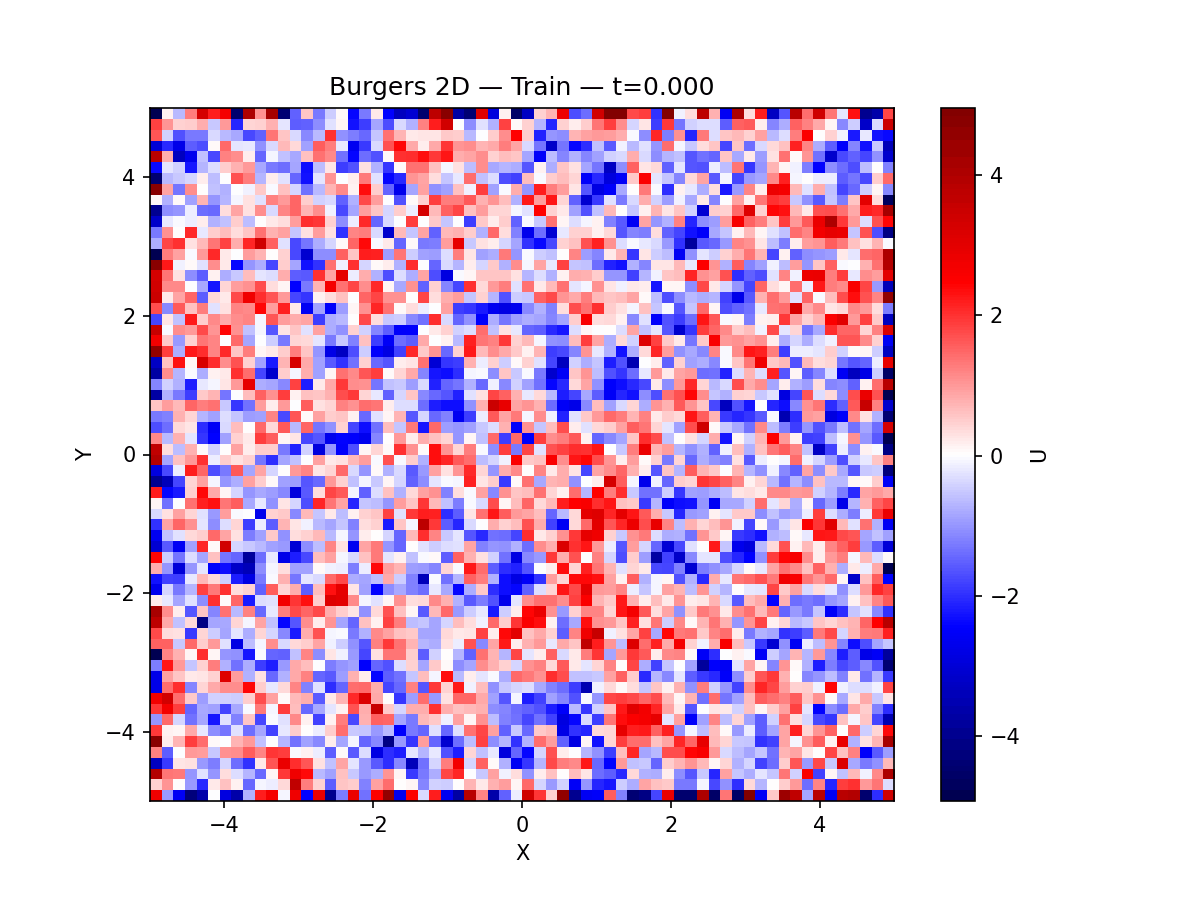
\includegraphics[width=0.72\textwidth]{images/2D_train_sample.png}
  \caption{Representative training sample from the 2D Burgers dataset ($\nu=0.05$, $64\times64$ grid). Each row shows one velocity component ($u$ top, $v$ bottom) at successive time steps. The diagonal shock structure illustrates the coupled 2D dynamics that the model must learn to reproduce autoregressively.}
  \label{fig:2d-train-sample}
\end{figure}

%==============================================================================
\section{Model Architecture}
\label{sec:2d_architecture}
%==============================================================================

The 2D model is derived from the 1D TCAN controller (Chapter~\ref{chap:approaches}) by replacing all 1D spatial operations with their 2D counterparts. The overall pipeline is identical: the model receives a history window of $W$ past fields and predicts the next field in an autoregressive rollout.

\paragraph{Input.}
The history window is a tensor of shape $(B, W, C, H, W_{\text{grid}})$, where $B$ is the batch size, $W$ is the number of past time steps, $C=2$ is the number of channels (velocity components), and $H \times W_{\text{grid}}$ is the spatial resolution.

\paragraph{Causal Temporal Attention (2D).}
As in the 1D case, a causal attention mechanism assigns learned importance weights to each past time step, restricting attention to the past. Spatial features at each time step are extracted with shared 2D convolutional layers before attention is computed.

\paragraph{FiLM Conditioning.}
The viscosity $\nu$ is injected as a scalar via a Feature-wise Linear Modulation (FiLM) layer, allowing the same weights to handle the full viscosity range.

\paragraph{Conv2D Decoder and Residual Correction.}
A stack of 2D convolutional layers maps the context vector back to a spatial field. The model predicts a bounded residual $\Delta u$, clipped via a tanh activation:
\[
  \hat{u}_{t+1} = u_t + \tanh\!\bigl(\Delta u_{\theta}(u_{t-W+1:t},\, \nu)\bigr).
\]
This residual formulation improves numerical stability during long rollouts. The complete pipeline is:
\[
  \underbrace{(B,W,C,H,W_{\text{grid}})}_{\text{History window}}
  \xrightarrow{\text{Causal Attn (2D)}}
  \xrightarrow{\text{FiLM}(\nu)}
  \xrightarrow{\text{Conv2D decoder}}
  \xrightarrow{\tanh\,\Delta}
  \underbrace{\hat{u}_{t+1}}_{\text{Next field}}.
\]

%==============================================================================
\section{Preliminary Results}
\label{sec:2d_results}
%==============================================================================

Training proceeded successfully in the sense that both training and validation losses decreased monotonically, confirming that gradient flow and optimization are stable for the 2D architecture. However, the model's spatial predictions remain qualitatively poor: it fails to reproduce the correct field structures and produces systematic low-frequency artifacts.

\begin{figure}[h!]
  \centering
  \begin{minipage}[t]{0.47\textwidth}
    \centering
    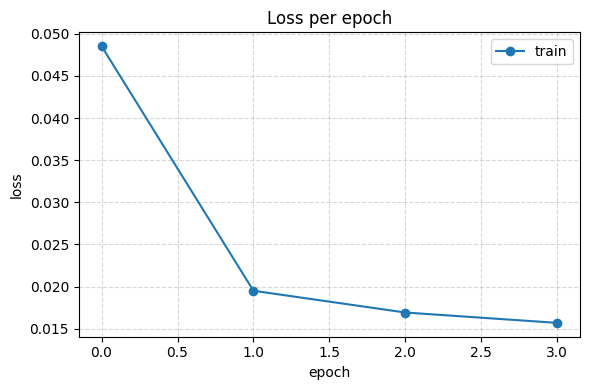
\includegraphics[width=\linewidth]{images/2D_loss.png}
    \caption{Training and validation loss curves for the 2D TCAN model over 100 epochs. Both curves decrease monotonically, confirming stable optimisation.}
    \label{fig:2d-loss}
  \end{minipage}\hfill
  \begin{minipage}[t]{0.47\textwidth}
    \centering
    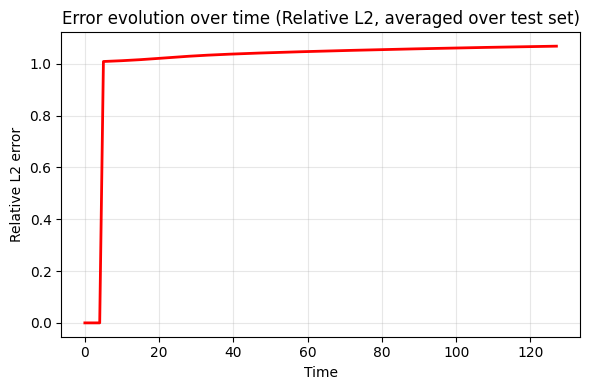
\includegraphics[width=\linewidth]{images/2D_output.png}
    \caption{Sample prediction from the 2D TCAN model after 100 epochs. Despite stable training, the predicted field (right) fails to reproduce the spatial structure of the ground truth (left), highlighting the remaining performance gap.}
    \label{fig:2d-output}
  \end{minipage}
\end{figure}

\begin{figure}[h!]
  \centering
  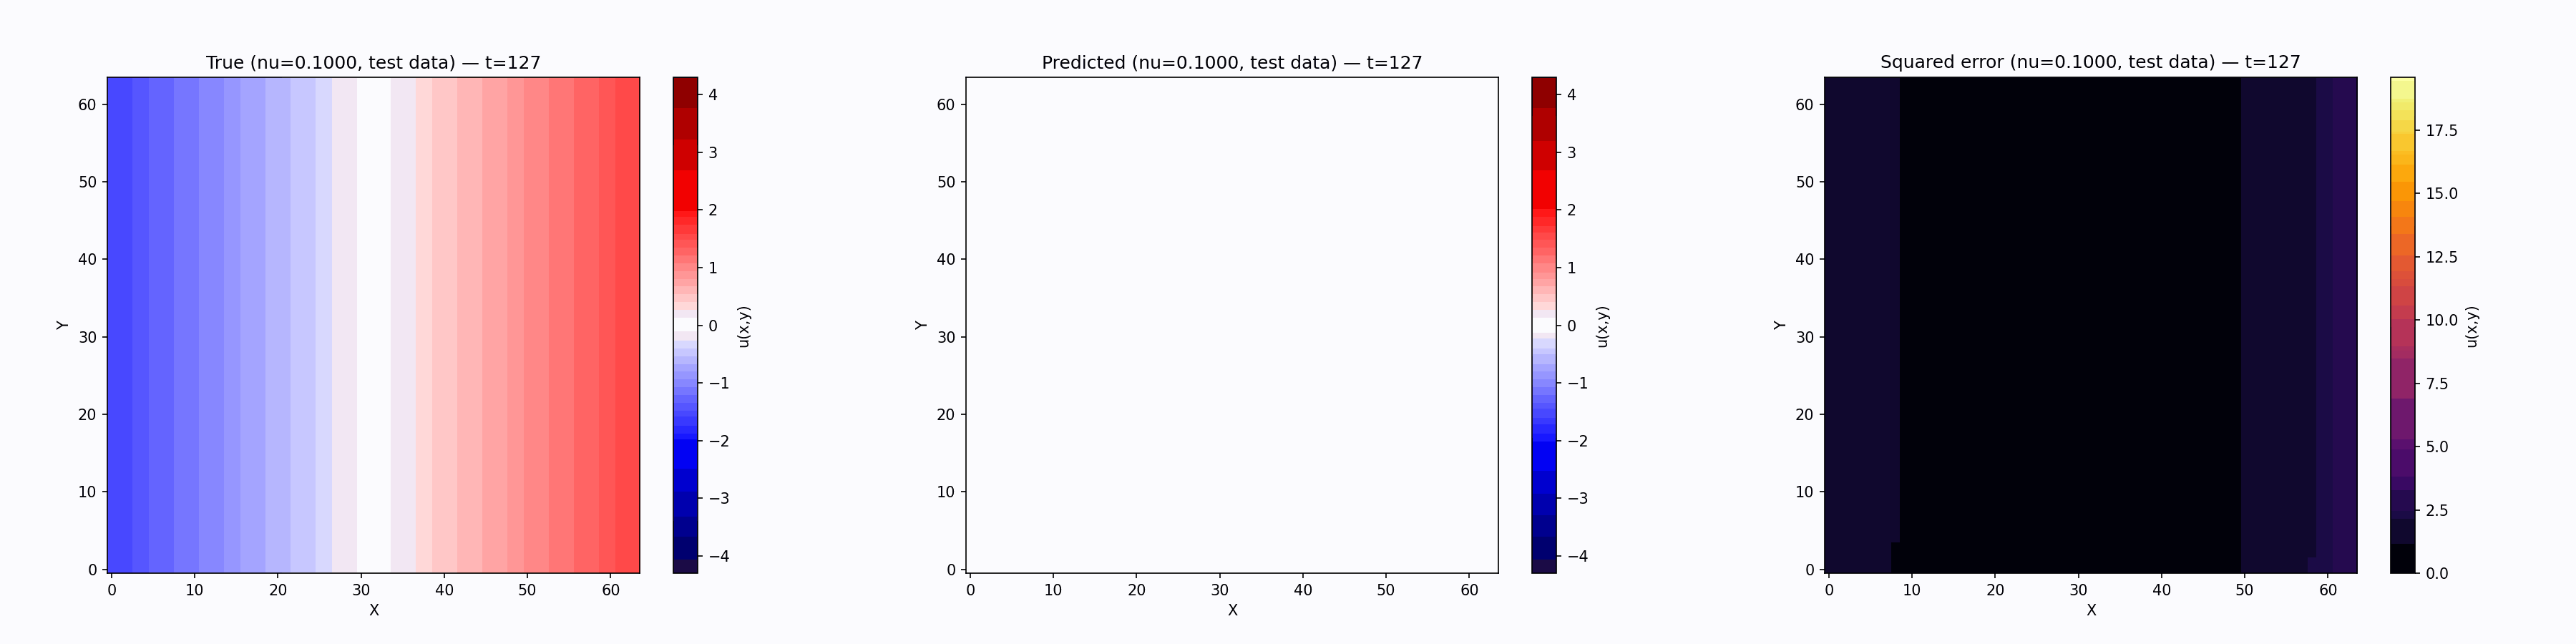
\includegraphics[width=0.80\textwidth]{images/2D_prediction_merged.png}
  \caption{Full rollout comparison for the 2D Burgers model at $\nu=0.1$: ground truth (top) vs.~TCAN prediction (bottom) across 16 time steps. The model captures the global structure but blurs sharp gradients, consistent with the low-frequency bias discussed in Section~\ref{sec:2d_results}.}
  \label{fig:2d-prediction-merged}
\end{figure}

The main factors contributing to this performance gap are:

\begin{enumerate}
    \item \textbf{Higher-dimensional input complexity}: The $(C, H, W)$ field has $2 \times 64 \times 64 = 8192$ values per snapshot, compared to 85--421 values in 1D. The model has fewer effective parameters per spatial degree of freedom.
    \item \textbf{Boundary condition mismatch}: The current implementation uses symmetric (reflect) padding, which does not match the periodic boundary conditions of the Burgers equation, introducing boundary artifacts that propagate inward during autoregressive rollout.
    \item \textbf{Autoregressive error accumulation}: As already observed in 1D, errors compound at each rollout step. The 2D case has more degrees of freedom, so accumulation is faster.
    \item \textbf{Limited training data}: The 2D dataset is substantially smaller than would be needed to cover the viscosity range and initial condition diversity at the same density as the 1D FNO dataset.
\end{enumerate}

%==============================================================================
\section{Planned Improvements and Next Steps}
\label{sec:2d_future_work}
%==============================================================================

Based on the analysis of the preliminary 2D results and the lessons from 1D TCAN, the following improvements are planned:

\paragraph{Boundary condition fix.}
Replace symmetric (reflect) padding with circular padding in all convolutional layers, which is the physically correct choice for a periodic domain.

\paragraph{Progressive rollout training.}
Apply the same progressive rollout curriculum used in 1D to stabilize training in the harder 2D regime. Scheduling exposure to the model's own prediction errors during training~\cite{lippe2023pde} is particularly relevant here.

\paragraph{Larger and more diverse 2D dataset.}
Scale up data generation using a pseudo-spectral solver at multiple resolutions, mirroring the 1D strategy. Active learning~\cite{musekamp2024active} can guide selection of the most informative samples.

\paragraph{Extension to incompressible Navier-Stokes.}
The incompressible Navier-Stokes equations extend the 2D Burgers system with a pressure term and an incompressibility constraint:
\begin{align}
  \frac{\partial \mathbf{u}}{\partial t} + (\mathbf{u} \cdot \nabla)\mathbf{u}
  &= -\nabla p + \nu \nabla^2 \mathbf{u}, \label{eq:ns_momentum} \\[4pt]
  \nabla \cdot \mathbf{u} &= 0. \label{eq:ns_incompressibility}
\end{align}
Handling the pressure field and enforcing the divergence-free condition require additional architectural adaptations (e.g.\ a Hodge-projection correction step), but the TCAN backbone and FiLM viscosity conditioning provide a natural starting point. Successfully extending the NFTM framework to Navier-Stokes would unlock realistic CFD applications at the scale of wing aerodynamics and turbulent channel flows.

